\begin{abstract}
In arbitrary-scale super-resolution, cell inputs are often motivated
by the size of a target pixel, but frequency ordering alone does
not establish what this readout computes. We evaluate recovery in
low-resolution Nyquist units and distinguish paired training ablations
from fixed-weight cell interventions. Normalisation reduces cross-scale
variation in all nine primary model--dataset groups and all 27 groups
including additional seeds; the original strict collapse criterion still
fails. Fixing image weights reduces variation on Set14 but increases it
on Urban100: pooled consistency does not imply image-wise consistency.
Coarse readout-loss
ordering replicates in four architecture--seed groups, yet a footprint
score has exactly the ranks of band index and scale averaging fails
function similarity in every group. A separately calibrated,
observation-only forecast also misses harmful interventions and does
not improve on a magnitude/spectrum baseline. These results support a
frequency-based evaluation coordinate while delimiting the tested readout
interpretations and instance-level guidance.
\end{abstract}
\begin{keywords}
Arbitrary-scale super-resolution, frequency recovery, cell conditioning,
readout diagnostics
\end{keywords}

\section{Introduction and Related Work}
\label{sec:intro}
Arbitrary-scale super-resolution (ASISR) predicts image values at continuous
coordinates. LIIF supplies a target cell size to a local decoder
\cite{chen2021liif}; LTE introduces cell-dependent phase estimation
\cite{lee2022lte}. Such conditioning can affect high-frequency errors,
but two questions are easily conflated: does a readout comparison exhibit
a frequency trend, and does that trend explain the computation or predict
when the readout is harmful? We study this distinction rather than
introducing another decoder.

Both the positive and negative roles of cell inputs have precedents.
LIIF already varies cell size at fixed queries and reports small
large-scale disadvantages in its ablation. IPE-LIIF integrates positional
features over a pixel and reports cases where an additional cell input
hurts \cite{liu2021ipe}. Thera provides analytic Gaussian filtering and
discusses a discrepancy between its theoretical filter and the bicubic
training degradation \cite{becker2025thera}. Thus cell intervention,
integrated encoding, harmful cell effects and filter mismatch are not
new principles here. Integration of intermediate features also need
not equal integration of a nonlinear decoder's final RGB output.

Frequency-resolved SR analysis likewise predates this work. HyRA studies
linear/nonlinear responses and frequency-spectrum similarity
\cite{fsds2024}, while texture-based error analysis goes beyond aggregate
PSNR \cite{magid2022texture}. Active sinusoidal probing also diagnoses
degradation mismatch \cite{kawai2026frequency}; Nyquist-normalised encoding
and spectral consistency appear in spatiotemporal forecasting
\cite{wang2026scaleanchoring}. Our fixed-checkpoint diagnostic normalises
reconstruction error by target signal energy and compares frequencies
in LR Nyquist units. Architecture/recipe effects are studied by a wider
continuous-SR retraining benchmark \cite{nasir2026empirical}; our fixed
checkpoints do not resolve that benchmark's general model comparison.
Generalized SURE \cite{eldar2008gsure} supplies risk estimates under stated
assumptions, whereas the bicubic proxy examined here has no unbiased-risk
guarantee.

Our contributions are two empirical tests with explicit simple controls.
First, we quantify the reduction in scale variation obtained by Nyquist
normalisation and distinguish image-wise variation from energy-weight
migration in pooled curves. Second, we distinguish coarse ordering, quantitative
prediction, function equivalence and harmful-intervention detection.
Replicated ordering coexists with failed stronger tests: it is not
evidence for a shared integral readout or a reliable instance-level
decision. The contribution is this controlled evidence and its limits,
not the first observation of harmful conditioning or a new risk theorem.

\section{Measurement and Comparison Design}
\label{sec:method}
\subsection{Separate sampling, target and conditioning}
Let $y=Ax$ be the LR observation of a continuous signal, $Q_hx$ the desired
measurement at a query coordinate $q$, and $c$ the cell supplied to
$F_\theta(y,q,c)$. Changing $A$, changing $Q_h$ and changing $c$ are
different interventions. Assigning $c=h$ does not prove that $F_\theta$
implements $Q_h$. Natural-image experiments use discrete HR targets and
bicubic antialiased LR preparation, not certified box averages of a known
field. Pixel-footprint arguments therefore motivate tests but do not
define ground truth in those experiments.

The evaluated LIIF/LTE/SC-INR variants inherit an EDSR-baseline encoder,
DIV2K training \cite{agustsson2017div2k}, 1000 epochs and training scales
$\times1$--$\times4$. SC-INR denotes the examined implementation with
sinc-modulated Fourier features; its phase/readout is not identified
with LTE's. A trained full/no-readout pair changes weights as well as
the readout path. A fixed-weight native/zero-cell comparison instead
changes only conditioning, and zero cell need not be in training support.
The LTE snapshot used in frozen-weight probes omits the extrapolation
cell clamp described in the original paper; conclusions concern these
checkpoints, not all published LTE implementations.

\subsection{Frequency recovery and scale variation}
For frequency band $b$, write $S_{ib}=\|\Pi_b(x_i-\bar x_i)\|^2$ and
$E_{ib}=\|\Pi_b(x_i-\hat x_i)\|^2$. Recovery relative to the centred zero
reconstruction is
\begin{equation}
 R_b=1-\frac{\sum_i E_{ib}}{\sum_i S_{ib}}.
 \label{eq:recovery}
\end{equation}
It can be negative and is not the equal-image mean of
$1-E_{ib}/S_{ib}$. The frequency study (L1) uses the RGB mean, unwindowed FFTs on centre
$240\times240$ crops, and Chebyshev frequency
$\nu=\max(|\nu_x|,|\nu_y|)$. It covers 14/30/30 images from
Set14/BSD100/Urban100 \cite{zeyde2010single,martin2001database,huang2015urban}.
Seven bins have edges $.25,.5,\ldots,2$ in $u=2s\nu$ for $s=2,3,4$;
the LR Nyquist boundary is $u=1$. The absolute-frequency control fixes
the same bins at $\nu=u/6$. Variation is
\begin{equation}
 D=\operatorname{median}_b\{\max_s R_b(s)-\min_s R_b(s)\}.
 \label{eq:variation}
\end{equation}
This compares two evaluation coordinates with different bin supports;
it does not prove equality of reconstructed functions.

\subsection{Readout losses and observation-only forecasts}
The paired training ablation and its replication (F1/G1) use centre HR256, 13/30/30 images, the RGB mean and three HR
frequency bands with cutoffs $1/8,1/4,1/2$. Their paired loss is
$L_b=R_b^{\rm full}-R_b^{\rm ablated}$; positive means the full model helps.
The footprint score $(.00006,.00552,.07235)$ and its replication criteria
were frozen before seed2/3 evaluation. Its three strictly increasing
values have exactly the same tied ranks as band index $(1,2,3)$.
The scale-average test (L2), with HR240 and 14/30/30 images, averages the full model over
31 conditioning scales $s'\in\{1,1.1,\ldots,4\}$ at fixed features and
coordinates. It tests the loss forecast and whether this averaged output
resembles the trained ablation. This operational average is not a
posterior over scale; HR truth enters its recovery score.

For the separate observation-only test, let $F_c,F_0$ be fixed-weight
native/zero-cell RGB outputs, $d=F_c-F_0$, and $B(y)$ bicubic upsampling.
True gain and the proxy forecast are
\begin{align}
 G&=\operatorname{MSE}(F_0,t)-\operatorname{MSE}(F_c,t),\\
 \hat G&=2\langle B(y)-F_0,d\rangle-\|d\|^2,\label{eq:proxy}\\
 G-\hat G&=2\langle t-B(y),d\rangle.\label{eq:bias}
\end{align}
Inner products and norms are pixel averages, optionally after band
projection. Equation~\eqref{eq:bias} is an elementary error identity:
unknown target/proxy error aligned with the correction changes its gain.
It is not an observation-only guarantee.

Calibration uses DIV2K train0001--0032; evaluation uses valid0825--0836,
centre HR128, $\times2/4$, no added noise, raw RGB outputs and shave4.
These interventions use one seed1 checkpoint per architecture.
One forecast uses Eq.~\eqref{eq:proxy}; another adds proxy alignment to
a calibrated ridge with scale/band indicators and observable change
energy, output/proxy energies and LR gradient/spectrum summaries. The
matched ridge baseline omits only alignment; standardisation is
calibration-only, with fixed ridge penalty 1 and an unpenalised intercept.
Band/scale median, energy-only, always-enable and always-disable controls
are also retained. All coefficients, forecasts and decisions were frozen
before evaluation scoring, with no test tuning. The evaluation images
were not used to fit these forecasts; their use in the original model
validation is not established. Forecasting requires both outputs and is
not a pre-inference shortcut.

\section{Results}
\label{sec:results}
\subsection{A useful coordinate, not a universal collapse law}
Nyquist normalisation reduces $D$ in all nine primary groups:
$.013$--$.061$ versus $.31$--$.46$ in absolute frequency.
Figure~\ref{fig:recovery} illustrates one successful dataset and the
Set14 exception; Table~\ref{tab:scale} retains all primary results.
The original criterion ($D\le.05$ in at least eight groups) fails,
with six of nine passing. This difference cannot be replaced by a
post-hoc relaxed tolerance.

\begin{figure}[t]
\centering
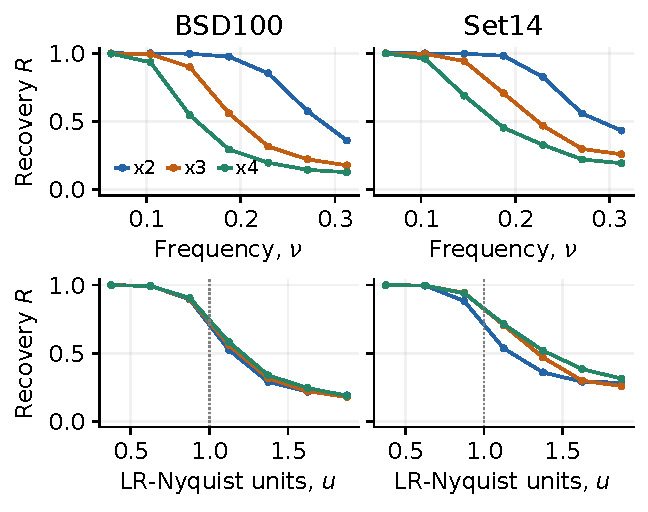
\includegraphics[width=\columnwidth]{figures/icassp-recovery.pdf}
\caption{SC-INR seed1: absolute-frequency (top) and LR-Nyquist (bottom)
recovery. All primary datasets enter Table~\ref{tab:scale}; these panels
show consistency on BSD100 and residual scale differences on Set14.
Recovery uses pooled energies, not a mean of image-wise scores.}
\label{fig:recovery}
\end{figure}
\begin{table}[t]\centering
\caption{Primary $D$ in LR-Nyquist units. All three Set14 entries fail
the original $.05$ tolerance.}\label{tab:scale}
\begin{tabular}{lccc}\toprule
Model & Set14 & BSD100 & Urban100\\\midrule
LIIF & .0586 & .0154 & .0165\\
LTE & .0548 & .0149 & .0190\\
SC-INR & .0605 & .0128 & .0147\\\bottomrule
\end{tabular}
\end{table}

A fixed descriptive sensitivity analysis reuses saved ring energies,
including two further seeds. Nyquist normalisation reduces $D$ in all
27 model--dataset--seed groups for every tested setting: the original
domain, below/above Nyquist subdomains, each leave-one-scale-out pair,
and pooled/equal-image aggregation (24 settings). These are dependent
comparisons, not 648 independent replications. In contrast, the strict
$.05$ tolerance passes 19/27 with original pooling and 27/27 with
equal-image averaging on the original domain. Thus the qualitative
normalisation benefit is stable here, while a strong collapse statement
depends on how images are weighted. The primary failure is retained.

To examine this dependence, let $R_{isb}=1-E_{isb}/S_{isb}$ and
$w_{isb}=S_{isb}/\sum_jS_{jsb}$. The pooled score is
$\sum_iw_{isb}R_{isb}$. A retrospective diagnostic holds weights fixed at
$\bar w_{ib}=\frac13\sum_sw_{isb}$, retaining all images and predictions.
This reduces $D$ in every Set14 group, from $.0493$--$.0616$ to
$.0227$--$.0294$, but increases it in every Urban100 group, from
$.0147$--$.0202$ to $.0293$--$.0538$; two Urban100 groups then exceed $.05$.
Weight migration can therefore amplify or conceal the measured variation.
It is not an independently identified physical cause: the same normalised
bin uses different HR frequencies at each scale, and $S$ enters both
the weights and individual scores.

Individual scores also remain dispersed: applying the same $.05$
tolerance descriptively gives only 7--9 of 14 images per Set14 group,
23--26 of 30 in BSD100, and 14--17 of 30 in Urban100. All nine original
Urban100 pooled curves pass, despite these image-wise exceptions.
These are dependent retrospective checks, not a new image-wise
pre-registered criterion. Fixed weights use HR spectra and are not an
observation-only selector; neither reweighting nor deleting an image
repairs the original failed criterion.

\subsection{Replicated ordering does not identify a readout}
Table~\ref{tab:readout} joins the four additional-seed tests. G1 meets
its $\rho\ge.5$ coarse-ordering threshold in all four groups; the high-band loss
exceeds the middle-band loss in 34/36 dataset--scale settings.
Equal-image aggregation gives 36/36 and correlations
$.641,.943,.646,.856$, preserving that weak conclusion. Per-image
recoveries permit this sensitivity check, but missing original per-image
energies prevent independent re-pooling of G1. The footprint formula
has no rank advantage over band index; multiplying by the proposed
recovery factor lowers correlation in all four groups.

\begin{table}[t]\centering
\caption{Paired training ablations. G1: loss correlation with band index
(identical to footprint ranks). L2: scale-average loss correlation,
median amplitude ratio on $L>.005$, and function similarity fraction.}
\label{tab:readout}
\begin{tabular}{lrrrr}\toprule
Group & G1 $\rho$ & L2 $\rho$ & Ratio & Similarity\\\midrule
LTE seed2 & .577 & .712 & .823 & .770\\
SC seed2 & .943 & .755 & .581 & .689\\
LTE seed3 & .676 & .954 & .833 & .748\\
SC seed3 & .885 & .700 & .337 & .653\\\bottomrule
\end{tabular}
\end{table}

L2 ordering ($\rho\ge.7$) passes 4/4 groups and its amplitude interval $[.5,2]$
passes 3/4. However, similarity (the ablation being closer to the averaged
than the full output) never reaches the frozen $.8$ threshold. L2 exceeds
the simpler footprint correlation by $.05$ in only 2/4 groups, both LTE,
below the required 3/4. Different crops/colour pooling mean G1 and L2
are interpreted within their own protocols; L2 superiority uses its
own recomputed footprint comparator, not the G1 column. High correlation does not
establish function equivalence or uniform quantitative superiority.

The intervention distinction is consequential even for the same image.
On barbara at $\times2$ in the high band, the trained SC full/ablation
pair has gain $-.193296$, while the fixed-weight native/zero-cell pair
has gain $+.009733$. These different comparisons cannot be pooled
as measurements of one mechanism. Known-field target/hint probes also
contain both gain signs within every band; their synthetic and
unsupported-query scope prevents a general natural-image causal claim.

\subsection{The tested forecasts miss harmful interventions}
For SC, 14 of 72 evaluation band outcomes are harmful
($G<-10^{-8}$), spanning nine images. Table~\ref{tab:negative} shows
that alignment does not add reliable discrimination over the matched
magnitude/spectrum baseline. The paired 12-image-cluster bootstrap
95\% interval for its balanced-accuracy improvement is
$[-.167,.143]$. LTE supplies just one harmful band outcome, so its high
apparent balanced accuracy cannot establish reliable negative detection.
Bands/scales share images; bootstrap intervals are marginal, not joint
95\% guarantees.

\begin{table}[t]\centering
\caption{SC harmful-band detection, 14 negatives/58 positives.
TP is detected harm; FP is beneficial output incorrectly flagged harmful;
BA is balanced accuracy.}
\label{tab:negative}
\begin{tabular}{lrrr}\toprule
Forecast & TP & FP & BA\\\midrule
Magnitude/spectrum ridge & 6 & 15 & .585\\
Ridge + alignment & 6 & 17 & .568\\
Bicubic proxy & 4 & 15 & .514\\\bottomrule
\end{tabular}
\end{table}

The original success gate requires at least 12 negatives on at least six
images, recall $\ge.75$,
precision $\ge.6$, false-positive rate $\le.25$, and an advantage over
every simple baseline (balanced accuracy by $.05$ and a positive paired
bootstrap lower bound). A separate full-RGB policy must reduce MSE
relative to every control with a positive lower bound. Both forecasts
choose native output iff the full-RGB forecast is positive, else zero-cell.
Both
fail the combined gate on both models. SC proxy policy reduces pooled
MSE by $1.31\times10^{-5}$ relative to always enabling, but its interval
$[-6.81\times10^{-6},4.78\times10^{-5}]$ crosses zero and mean PSNR falls
$.0047$ dB. The alignment policy is slightly worse in MSE. These are
not adaptive benefits hidden by the classification threshold.

Saved-output checks with shave0/4/8 retain SC harm in 16/14/14 original
band outcomes and 6/5/5 full-RGB outcomes; LTE has 1/1/1 harmful bands
and no harmful RGB outcome. Two fixed alternative band partitions give
10--16 harmful SC outcomes; harm is not confined to the original cutoffs.
These post-evaluation sensitivity checks do not refit forecasts or claim
new confirmation. The original fixed RGB policies still lack a reliable
SC improvement at every shave; the LTE proxy policy is harmful throughout.

\section{Implications and Limits}
LR-Nyquist frequency is useful for comparing recovery across scales,
but pooled consistency also depends on image weights and can hide
image-wise exceptions. Reweighting has opposite effects across datasets;
it is not a universal correction. Readout evaluation should report signed gains and
simple band controls; rank correlation with a three-valued predictor
cannot validate its quantitative form. Training ablations and
fixed-weight conditioning answer different questions and can give
opposite signs. Within these checkpoints, the tested proxy adds no
reliable harmful-intervention guidance; this does not exclude better
proxies or mechanisms.

\newpage
Scope is limited to the inherited recipes, crops, scales and three seeds.
There is no fair performance benchmark against all integrated-readout
methods, no certified physical HR footprint, and no universal decoder
limit. Zero-cell/synthetic queries introduce support differences. All
primary failures and saved outputs are retained; independent numerical
audits verify scoring, not a new model implementation. The new natural
forecast test takes 224.19 seconds on one CPU thread, with no GPU or SR
training; offline robustness adds no inference. Its cost includes both
native and zero-cell predictions. These results establish a controlled
empirical baseline; a predictive rule needs separate validation.

\section{Conclusion}
Frequency normalisation yields a robust reduction in measured scale
variation, whereas pooled consistency need not hold image-wise. Coarse
readout ordering replicates, but footprint ranking has no advantage
over band index and does not validate
the stronger function or harmful-benefit forecasts examined here.
Separating these evidence levels makes ASISR readout claims testable
without treating correlations as mechanisms.

\section{Acknowledgments}
Claude and OpenAI Codex assisted with text, analysis code, figures and
record checks in Sections 1--5. Results were checked against stored
records; scoring audits are not model reimplementations. Human author
review and responsibility are required before submission.
